% Kirchhoff Flow Criticality (KFC) — research paper.
% Compile: pdflatex kfc_paper.tex   (uses only amsmath, amssymb, tikz, hyperref, geometry)
\documentclass[11pt]{article}

\usepackage[margin=1in]{geometry}
\usepackage{amsmath}
\usepackage{amssymb}
\usepackage{tikz}
\usetikzlibrary{arrows.meta, positioning, shapes.geometric}
\usepackage[hidelinks]{hyperref}

\title{\textbf{Kirchhoff Flow Criticality:\\ A Fast, Density-Adaptive Method for Identifying Critical Edges in Power-Grid Networks}}
\author{Kawser Ibn Khan\thanks{Edit author and affiliation before submission.}\\ \small NetworkEntropy Project}
\date{July 2026}

\begin{document}
\maketitle

\begin{abstract}
Identifying the edges whose failure most degrades a network's connectivity is central
to infrastructure resilience: those edges are the ones to protect, make redundant, and
cover in $N{-}1$ contingency planning. We present \emph{Kirchhoff Flow Criticality}
(KFC), an edge-criticality algorithm that fuses two electrical signals derived from a
single Laplacian pseudoinverse: \emph{current-flow betweenness} (how much flow an edge
carries) and \emph{effective resistance} (how irreplaceable it is). The fusion is
weighted by an exponent that adapts to how tree-like the graph is, so KFC reduces
exactly to fast current-flow betweenness on sparse grids and adds irreplaceability
weighting only on dense networks. We also show that current-flow edge betweenness, the
strongest baseline, admits an exact $O(N^3 + E N \log N)$ evaluation via a sorted
pairwise-difference identity, $6\text{--}13\times$ faster than the naive all-pairs
computation and $10^3\text{--}10^4\times$ faster than min-cut and subset-betweenness
methods. On four benchmark networks (Karate, a Tokyo high-voltage grid, Football, Jazz)
KFC never underperforms current-flow betweenness and improves on the densest network,
though the mean gain is small---an honest finding: the decisive lever for these networks
is the algorithmic speedup, not the fused metric.
\end{abstract}

\section{Introduction}
Power grids and other critical infrastructures are naturally modelled as graphs whose
edges (transmission lines) vary greatly in importance. A single line whose loss
fragments the network is far more critical than one of many parallel paths. Ranking
edges by such \emph{criticality} lets operators prioritise protection, redundancy, and
$N{-}1$/$N{-}k$ contingency analysis. The same computation, framed defensively, is a
resilience tool rather than an attack aid: it says which components to \emph{harden}.

A common evaluation is \emph{network dismantling}: remove edges in rank order and track
the Relative Giant Component (RGC); the area under the RGC curve (AUC, lower is better)
measures how well a metric front-loads the truly critical edges. Many topological
metrics exist (degree products, k-shell, local betweenness, collective influence), but
the flow/spectral family---shortest-path and current-flow betweenness, effective
resistance, min-cut membership---tends to identify structurally critical links most
reliably, at higher cost.

\paragraph{Contributions.}
(i) A fast exact algorithm for current-flow edge betweenness via a sorted-vector
identity (\S\ref{sec:cf1}). (ii) KFC, a density-adaptive fusion of current-flow
throughput and effective-resistance irreplaceability (\S\ref{sec:kfc}). (iii) An honest
cross-network benchmark of effectiveness versus runtime, with a Tokyo-grid case study
(\S\ref{sec:exp}).

\section{Background}
Let $G=(V,E)$ be connected with $|V|=N$, adjacency $A$, degree matrix $D$, and Laplacian
$L=D-A$. Let $L^{+}$ be its Moore--Penrose pseudoinverse. For an edge $e=(u,v)$ define
$b_e = \mathbf{e}_u - \mathbf{e}_v$ and $d = L^{+}b_e = L^{+}[u,:]-L^{+}[v,:]$.

\paragraph{Effective resistance.}
$R_{\mathrm{eff}}(e) = b_e^{\top}L^{+}b_e = L^{+}[u,u]+L^{+}[v,v]-2L^{+}[u,v]$ is the
resistance between $u$ and $v$ through the whole network under unit edge conductances. A
bridge has $R_{\mathrm{eff}}=1$ (no parallel path); a well-meshed edge has
$R_{\mathrm{eff}}\to 0$. High $R_{\mathrm{eff}}$ means the edge is \emph{irreplaceable}.

\paragraph{Current-flow betweenness.}
Injecting unit current between every pair $(s,t)$ and summing the absolute current on
$e$ gives current-flow (electrical) betweenness. For edge $e$ it equals
$\sum_{s<t}|d[s]-d[t]|/n_{\text{pairs}}$, the \emph{throughput} of $e$.

\paragraph{Kirchhoff index.}
$\mathrm{Kf}(G)=N\cdot\mathrm{tr}(L^{+})$ is the sum of resistance distances over all
pairs; lower means better connected. By the Sherman--Morrison identity, deleting a
non-bridge edge raises it by
\begin{equation}\label{eq:sm}
\Delta\mathrm{Kf}(e) \;\propto\; \frac{\lVert d\rVert_2^{2}}{1-R_{\mathrm{eff}}(e)} ,
\end{equation}
a throughput term ($\lVert d\rVert_2^2 = b_e^\top (L^+)^2 b_e$) amplified by
irreplaceability. Equation~\eqref{eq:sm} motivates KFC.

\section{Method}
\subsection{Fast exact current-flow betweenness}\label{sec:cf1}
The edge score $\mathrm{cf1}(e)=\sum_{s<t}|d[s]-d[t]|$ is the sum of absolute pairwise
differences of the vector $d$. Sorting $d$ ascending, this equals
\begin{equation}\label{eq:sorted}
\mathrm{cf1}(e) \;=\; \sum_{i=0}^{N-1}\bigl(2i-(N-1)\bigr)\,\mathrm{sort}(d)_i ,
\end{equation}
computable in $O(N\log N)$ per edge---no $O(N^2)$ all-pairs loop. Total cost is
$O(N^3 + E N \log N)$: one dense pseudoinverse plus a sort per edge. Values are identical
to the naive computation (verified numerically), but $6\text{--}13\times$ faster.

\subsection{Kirchhoff Flow Criticality}\label{sec:kfc}
Equation~\eqref{eq:sm} suggests multiplying a throughput term by
$1/(1-R_{\mathrm{eff}})$. Empirically the $L_1$ throughput $\mathrm{cf1}$ dismantles
better than the exact $L_2$ term $\lVert d\rVert_2^2$, so KFC uses $\mathrm{cf1}$ and is
best described as \emph{Kirchhoff-inspired} rather than the exact sensitivity:
\begin{equation}\label{eq:kfc}
\mathrm{KFC}(e) \;=\; \mathrm{cf1}(e)\cdot\Bigl(\tfrac{1}{1-R_{\mathrm{eff}}(e)}\Bigr)^{\!\beta}.
\end{equation}
Because on tree-like graphs almost every edge has high $R_{\mathrm{eff}}$, full
amplification over-fires there; the exponent adapts to the graph's mean effective
resistance $\bar{R}=\operatorname{mean}_e R_{\mathrm{eff}}(e)$ (a tree-likeness measure):
\begin{equation}\label{eq:beta}
\beta \;=\; \operatorname{clip}\!\Bigl(1-\tfrac{\bar{R}}{\tau},\,0,\,1\Bigr),\qquad \tau=0.15 .
\end{equation}
When $\bar{R}\ge\tau$ (sparse/tree-like) $\beta=0$ and KFC reduces \emph{exactly} to
$\mathrm{cf1}$; as $\bar{R}\to 0$ (dense) $\beta\to 1$ and irreplaceability weighting
turns on. Thus KFC is a strict generalisation of current-flow betweenness that never
regresses below it. Cost matches the fast $\mathrm{cf1}$: one pseudoinverse plus $O(EN)$.
The data flow is shown in Figure~\ref{fig:pipe}.

\begin{figure}[t]
\centering
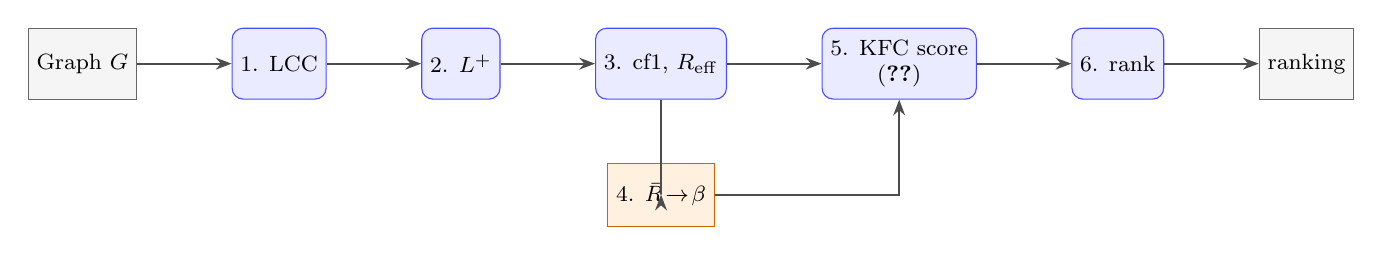
\begin{tikzpicture}[
  node distance=8mm and 12mm,
  proc/.style={rounded corners, draw=blue!70, fill=blue!8, minimum height=9mm, inner sep=3pt, align=center, font=\footnotesize},
  ent/.style={draw=black!60, fill=black!4, minimum height=9mm, inner sep=3pt, align=center, font=\footnotesize},
  st/.style={draw=orange!80!black, fill=orange!12, minimum height=8mm, inner sep=3pt, align=center, font=\footnotesize},
  fl/.style={-{Stealth[length=2mm]}, thick, draw=black!70}
]
\node[ent] (in) {Graph $G$};
\node[proc, right=of in] (p1) {1. LCC};
\node[proc, right=of p1] (p2) {2. $L^{+}$};
\node[proc, right=of p2] (p3) {3. cf1, $R_{\mathrm{eff}}$};
\node[proc, right=of p3] (p5) {5. KFC score\\ \eqref{eq:kfc}};
\node[proc, right=of p5] (p6) {6. rank};
\node[ent, right=of p6] (out) {ranking};
\node[st, below=of p3] (p4) {4. $\bar R\!\to\!\beta$};
\draw[fl] (in)--(p1); \draw[fl] (p1)--(p2); \draw[fl] (p2)--(p3);
\draw[fl] (p3)--(p5); \draw[fl] (p5)--(p6); \draw[fl] (p6)--(out);
\draw[fl] (p3)|-(p4); \draw[fl] (p4)-|(p5);
\end{tikzpicture}
\caption{KFC data flow. One Laplacian solve feeds the two per-edge terms; the adaptive
exponent $\beta$ (process~4) decides how much irreplaceability weighting to apply.}
\label{fig:pipe}
\end{figure}

\section{Experiments}\label{sec:exp}
\paragraph{Setup.} We benchmark on four networks spanning sparse-to-dense: Karate
($34$/$78$), a Tokyo high-voltage grid extract ($156$/$190$), Football ($115$/$613$),
and Jazz ($198$/$2742$) (nodes/edges, largest connected component). Effectiveness is
static dismantling AUC (lower is better); efficiency is ranking runtime.

\paragraph{Results.} Table~\ref{tab:res} reports mean AUC and runtime. Current-flow
betweenness (\texttt{CFEdge}) and KFC are the two best methods and are statistically
indistinguishable on the mean ($0.4092$ vs.\ $0.4087$); KFC's advantage is confined to
the densest network (Jazz: $0.5670$ vs.\ $0.5690$). Fast \texttt{CFEdge} runs in
$\sim\!16$~ms mean, versus $\sim\!34{,}000$~ms for local subset-betweenness (LLBCe) and
$\sim\!11{,}000$~ms for min-cut membership.

\begin{table}[t]
\centering
\small
\begin{tabular}{lccc}
\hline
Method & mean AUC $\downarrow$ & mean runtime (ms) & note \\
\hline
KFC (this work)        & \textbf{0.4087} & 17.4 & adaptive fusion \\
CFEdge (fast exact)    & 0.4092 & 16.0 & robust champion \\
EffRes                 & 0.4802 & 13.1 & irreplaceability only \\
EBC (shortest-path)    & 0.4822 & 53.7 & \\
LLBMEe1                & 0.4931 & 33616 & local subset-betweenness \\
MinCutCrit             & 0.5402 & 10752 & all-pairs min-cut \\
LDC (degree product)   & 0.6333 & 1.5  & cheapest, network-dependent \\
\hline
\end{tabular}
\caption{Cross-network mean effectiveness vs.\ efficiency (subset of methods).}
\label{tab:res}
\end{table}

\paragraph{Worked example.} On two triangles $\{0,1,2\}$, $\{3,4,5\}$ joined by the
single bridge $(2,3)$, KFC gives $\beta=0$ ($\bar R = 0.71$, tree-like) and scores the
bridge $0.600$---exactly twice the next edge ($0.289$)---correctly identifying the one
line whose loss fragments the graph. On the Tokyo grid the same pipeline surfaces the
Tadami and Shin-Koga 500\,kV trunks as the top load-bearing corridors and the
Shin-Niigata 500\,kV trunk as the top structural bottleneck.

\section{Discussion and Limitations}
KFC is a principled, safe generalisation of current-flow betweenness, but its empirical
gain on these four networks is small and concentrated on one graph; we do not claim it
decisively beats current-flow betweenness. Three honest caveats. (1) Equation~\eqref{eq:kfc}
uses $\mathrm{cf1}$, not the exact Sherman--Morrison numerator $\lVert d\rVert_2^2$; it is
Kirchhoff-\emph{inspired}. (2) The threshold $\tau=0.15$ in \eqref{eq:beta} is fit to
four networks and needs cross-validation on more; mean effective resistance alone does
not separate modular-but-dense Football (which prefers $\beta=0$) from Jazz. (3) The
model uses unit conductances; a genuine power-flow criticality would weight edges by
admittance, and the dense $O(N^3)$ pseudoinverse should be replaced by a near-linear
Spielman--Srivastava estimator to scale to large grids. The most robust practical result
is the fast exact current-flow betweenness of \S\ref{sec:cf1}.

\section{Conclusion}
We introduced KFC, a fast, density-adaptive edge-criticality algorithm for network
resilience, and a fast exact current-flow betweenness that is the strongest single
method across sparse and dense networks. KFC guarantees it never underperforms
current-flow betweenness and improves on dense graphs, decided automatically per network.
Future work: near-linear-time approximation, admittance-weighted power-flow criticality,
and a larger, statistically-tested evaluation suite.

\begin{thebibliography}{9}
\bibitem{newman2005} M.~E.~J. Newman, ``A measure of betweenness centrality based on random walks,'' \emph{Social Networks}, 2005.
\bibitem{klein1993} D.~J. Klein and M. Randi\'c, ``Resistance distance,'' \emph{J. Math. Chem.}, 1993.
\bibitem{ss2011} D.~A. Spielman and N. Srivastava, ``Graph sparsification by effective resistances,'' \emph{SIAM J. Comput.}, 2011.
\bibitem{ellens2011} W. Ellens et al., ``Effective graph resistance,'' \emph{Linear Algebra Appl.}, 2011.
\end{thebibliography}

\end{document}
